\documentclass{article}
%%%%%%%%%%%%%%%%%%%%%%%%%%%%%%%%%%%%%%%%%
% Lachaise Assignment
% Structure Specification File
% Version 1.0 (26/6/2018)
%
% This template originates from:
% http://www.LaTeXTemplates.com
%
% Authors:
% Marion Lachaise & François Févotte
% Vel (vel@LaTeXTemplates.com)
%
% License:
% CC BY-NC-SA 3.0 (http://creativecommons.org/licenses/by-nc-sa/3.0/)
% 
%%%%%%%%%%%%%%%%%%%%%%%%%%%%%%%%%%%%%%%%%

%----------------------------------------------------------------------------------------
%	PACKAGES AND OTHER DOCUMENT CONFIGURATIONS
%----------------------------------------------------------------------------------------

\usepackage{amsmath,amsfonts,stmaryrd,amssymb,subcaption} % Math packages

\usepackage{enumerate} % Custom item numbers for enumerations

\usepackage[ruled]{algorithm2e} % Algorithms

\usepackage[framemethod=tikz]{mdframed} % Allows defining custom boxed/framed environments

\usepackage{listings} % File listings, with syntax highlighting
\lstset{
	basicstyle=\ttfamily, % Typeset listings in monospace font
}

\usepackage{hyperref}

%----------------------------------------------------------------------------------------
%	DOCUMENT MARGINS
%----------------------------------------------------------------------------------------

\usepackage{geometry} % Required for adjusting page dimensions and margins

\geometry{
	paper=a4paper, % Paper size, change to letterpaper for US letter size
	top=2.5cm, % Top margin
	bottom=2.5cm, % Bottom margin
	left=2.5cm, % Left margin
	right=2.5cm, % Right margin
	headheight=14pt, % Header height
	footskip=1.5cm, % Space from the bottom margin to the baseline of the footer
	headsep=1.2cm, % Space from the top margin to the baseline of the header
	%showframe, % Uncomment to show how the type block is set on the page
}

%----------------------------------------------------------------------------------------
%	FONTS
%----------------------------------------------------------------------------------------

\usepackage[utf8]{inputenc} % Required for inputting international characters
\usepackage[T1]{fontenc} % Output font encoding for international characters

\usepackage{XCharter} % Use the XCharter fonts

%----------------------------------------------------------------------------------------
%	COMMAND LINE ENVIRONMENT
%----------------------------------------------------------------------------------------

% Usage:
% \begin{commandline}
%	\begin{verbatim}
%		$ ls
%		
%		Applications	Desktop	...
%	\end{verbatim}
% \end{commandline}

\mdfdefinestyle{commandline}{
	leftmargin=10pt,
	rightmargin=10pt,
	innerleftmargin=15pt,
	middlelinecolor=black!50!white,
	middlelinewidth=2pt,
	frametitlerule=false,
	backgroundcolor=black!5!white,
	frametitle={Command Line},
	frametitlefont={\normalfont\sffamily\color{white}\hspace{-1em}},
	frametitlebackgroundcolor=black!50!white,
	nobreak,
}

% Define a custom environment for command-line snapshots
\newenvironment{commandline}{
	\medskip
	\begin{mdframed}[style=commandline]
}{
	\end{mdframed}
	\medskip
}

%----------------------------------------------------------------------------------------
%	FILE CONTENTS ENVIRONMENT
%----------------------------------------------------------------------------------------

% Usage:
% \begin{file}[optional filename, defaults to "File"]
%	File contents, for example, with a listings environment
% \end{file}

\mdfdefinestyle{file}{
	innertopmargin=1.6\baselineskip,
	innerbottommargin=0.8\baselineskip,
	topline=false, bottomline=false,
	leftline=false, rightline=false,
	leftmargin=2cm,
	rightmargin=2cm,
	singleextra={%
		\draw[fill=black!10!white](P)++(0,-1.2em)rectangle(P-|O);
		\node[anchor=north west]
		at(P-|O){\ttfamily\mdfilename};
		%
		\def\l{3em}
		\draw(O-|P)++(-\l,0)--++(\l,\l)--(P)--(P-|O)--(O)--cycle;
		\draw(O-|P)++(-\l,0)--++(0,\l)--++(\l,0);
	},
	nobreak,
}

% Define a custom environment for file contents
\newenvironment{file}[1][File]{ % Set the default filename to "File"
	\medskip
	\newcommand{\mdfilename}{#1}
	\begin{mdframed}[style=file]
}{
	\end{mdframed}
	\medskip
}

%----------------------------------------------------------------------------------------
%	NUMBERED QUESTIONS ENVIRONMENT
%----------------------------------------------------------------------------------------

% Usage:
% \begin{question}[optional title]
%	Question contents
% \end{question}

\mdfdefinestyle{question}{
	innertopmargin=1.2\baselineskip,
	innerbottommargin=0.8\baselineskip,
	roundcorner=5pt,
	nobreak,
	singleextra={%
		\draw(P-|O)node[xshift=1em,anchor=west,fill=white,draw,rounded corners=5pt]{%
		Question \theQuestion\questionTitle};
	},
}

\newcounter{Question} % Stores the current question number that gets iterated with each new question

% Define a custom environment for numbered questions
\newenvironment{question}[1][\unskip]{
	\bigskip
	\stepcounter{Question}
	\newcommand{\questionTitle}{~#1}
	\begin{mdframed}[style=question]
}{
	\end{mdframed}
	\medskip
}

%----------------------------------------------------------------------------------------
%	WARNING TEXT ENVIRONMENT
%----------------------------------------------------------------------------------------

% Usage:
% \begin{warn}[optional title, defaults to "Warning:"]
%	Contents
% \end{warn}

\mdfdefinestyle{warning}{
	topline=false, bottomline=false,
	leftline=false, rightline=false,
	nobreak,
	singleextra={%
		\draw(P-|O)++(-0.5em,0)node(tmp1){};
		\draw(P-|O)++(0.5em,0)node(tmp2){};
		\fill[black,rotate around={45:(P-|O)}](tmp1)rectangle(tmp2);
		\node at(P-|O){\color{white}\scriptsize\bf !};
		\draw[very thick](P-|O)++(0,-1em)--(O);%--(O-|P);
	}
}

% Define a custom environment for warning text
\newenvironment{warn}[1][Warning:]{ % Set the default warning to "Warning:"
	\medskip
	\begin{mdframed}[style=warning]
		\noindent{\textbf{#1}}
}{
	\end{mdframed}
}

%----------------------------------------------------------------------------------------
%	INFORMATION ENVIRONMENT
%----------------------------------------------------------------------------------------

% Usage:
% \begin{info}[optional title, defaults to "Info:"]
% 	contents
% 	\end{info}

\mdfdefinestyle{info}{%
	topline=false, bottomline=false,
	leftline=false, rightline=false,
	nobreak,
	singleextra={%
		\fill[black](P-|O)circle[radius=0.4em];
		\node at(P-|O){\color{white}\scriptsize\bf i};
		\draw[very thick](P-|O)++(0,-0.8em)--(O);%--(O-|P);
	}
}

% Define a custom environment for information
\newenvironment{info}[1][Info:]{ % Set the default title to "Info:"
	\medskip
	\begin{mdframed}[style=info]
		\noindent{\textbf{#1}}
}{
	\end{mdframed}
}
 % Include the file specifying the document structure and custom commands

\title{SI 649: Communication Visualization Project \\ Static Blog Post} % Title of the assignment

\author{Mingliang Duanmu\\ \texttt{duanmuml@umich.edu}} % Author name and email address

\date{\today} % University, school and/or department name(s) and a date

\begin{document}

\maketitle % Print the title

\section{Learning Objectives}

The viewer will be able to:
\begin{itemize}
    \item \textbf{Compare} the natural amenity rating and geographic distribution across different states in the US.
    \item \textbf{Conclude} the diseases with highest mortality in Red Lake County and the trend of mortality during the past 30 years.
    \item \textbf{Contrast} the unemployment rate, average household income, and poverty rate of Red Lake County to the national and state-level data.
    \item \textbf{Observe} the difference between educational resources within the state of Minnesota.
\end{itemize}

\section{Design Process}

\subsection*{Idea}

Most of my ideas of building the visualizations are based on the aspects mentioned by the author in the article "I called this place ‘America’s worst place to live.’ Then I went there". The static version of my visualization focuses on comparisons of Red Lake County statistics against national average or counties within the same state. I apply various methods of encoding, representation and annotation to make it quick for readers to notice the contrast. I also go a little beyond to display extra aspects of Red Lake County that add to a more complete impression of the place for readers.

\subsection*{Data}

I search extensively online to find useful and credible datasets for my visualizations. The data sources include Kaggle (the mortality data, public school data), USDA (natural amenity), U.S. Census Bureau (poverty and household income), U.S. Bureau of Labor Statistics (unemployment rate). \\
\noindent
Based on the date of the article, all my visualizations are based on the data before 2015. I do some data cleaning and filtering on the raw data to kick out wrong values and useless information, as well as reorganizing structures of tables to make them more suitable to Altair grammar.

\subsection*{Tool}

I use both Altair and Tableau for my static visualizations. Tableau is convenient for plotting map graphs while Altair has more freedom of customizing all the parameters of a graph, together with versatility to add layers and organize multiple subplots. Also, my interactive visualizations can be directly built upon the static Altair graphs. Personally, I prefer programming-based tools instead of software with rich GUI that requires more learning cost.

\subsection*{Visualizations}

\subsubsection*{Map graph of national natural amenity distribution}

First things first, I focus on the most important fact that leads to the conclusion of "America’s worst place to live", which is the natural amenity rating. I think using a map graph showing geographical difference and distribution of such an index is the most clear and straightforward way. \\
\begin{figure}[htbp]
    \centering
    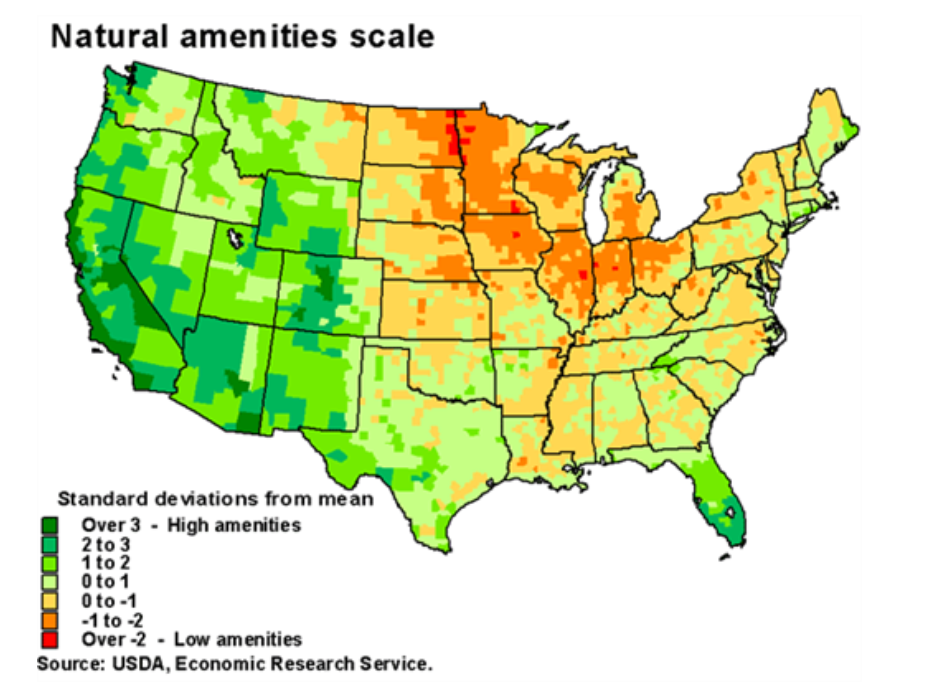
\includegraphics[scale=0.6]{NA_ins.png}
    \caption{Colored choropleth map on \href{https://www.ers.usda.gov/data-products/natural-amenities-scale/}{USDA}}
\end{figure} \\
\noindent 
At first I wanted to use Altair for plotting a colored choropleth map inspired by Figure 1, however due to the lack of documentation and tutorials, together with Altair's inability of making zoom interactions on the map graphs, I switched to Tableau for this plot in Figure 2. \\
\begin{figure}[htbp]
    \centering
    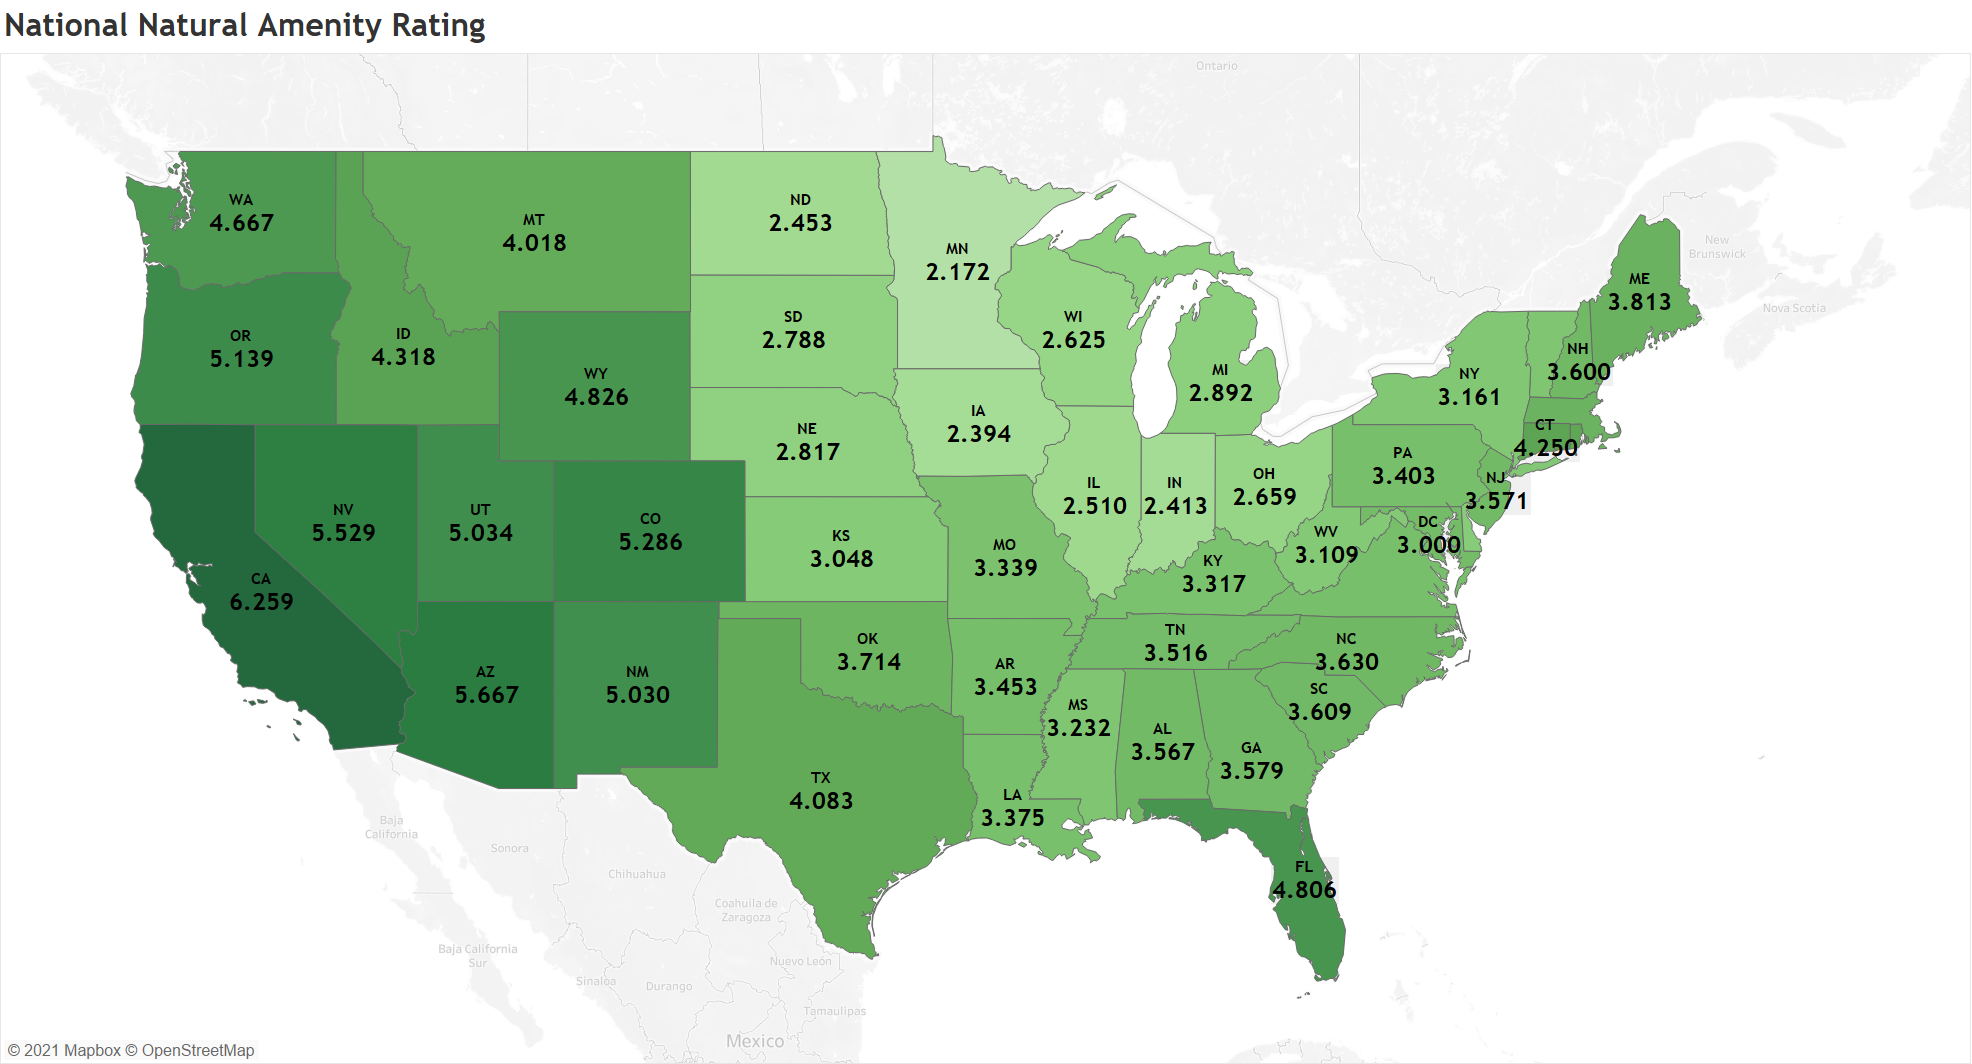
\includegraphics[scale=0.4]{NA.png}
    \caption{My colored choropleth map created by Tableau}
\end{figure} \\
\noindent
Figure 3 is my failed attempt to encode values in color in Altair, I can only draw scatter plots using longitude and latitude of each county. \\
\begin{figure}[htbp]
    \centering
    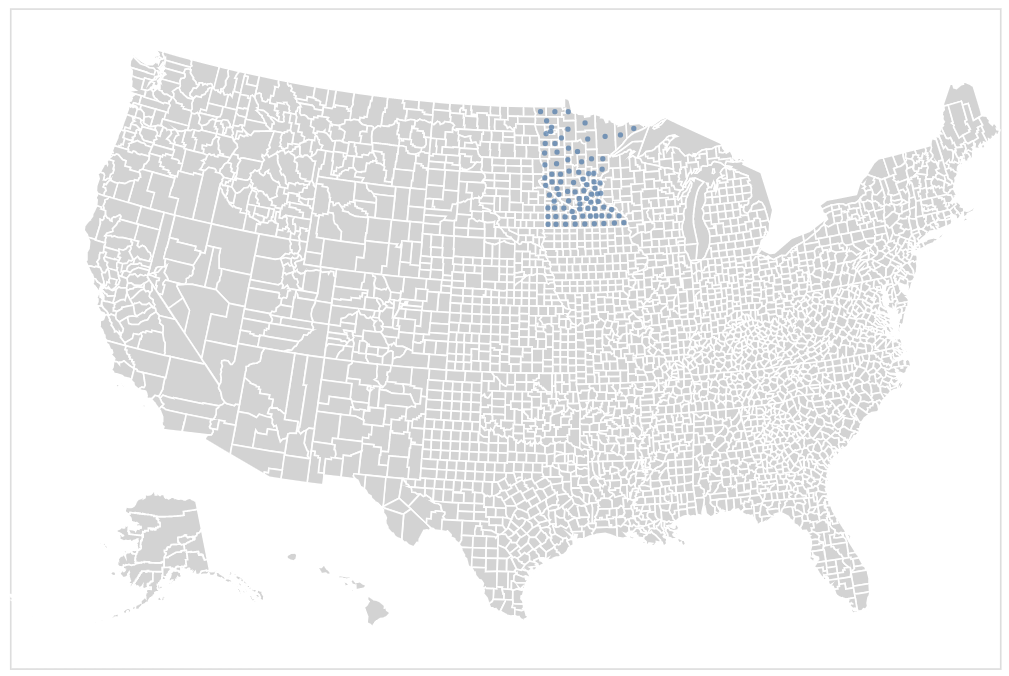
\includegraphics[scale=0.3]{NA_att.png}
    \caption{I cannot figure out how to plot data on map using Altair}
\end{figure}

\subsubsection*{Line \& scatter plot of unemployment rate, average household income, and poverty rate}

Since the author claims that Red Lake County does a good job by economic metrics regarding unemployment rate, average household income and poverty rate, I decide to use scatter plot to compare them to other counties within the state, as well as the national data. While the unemployment rate I find only applies to each state, I use a line plot to compare it with the national data. \\
\begin{figure}[htbp]
    \centering
    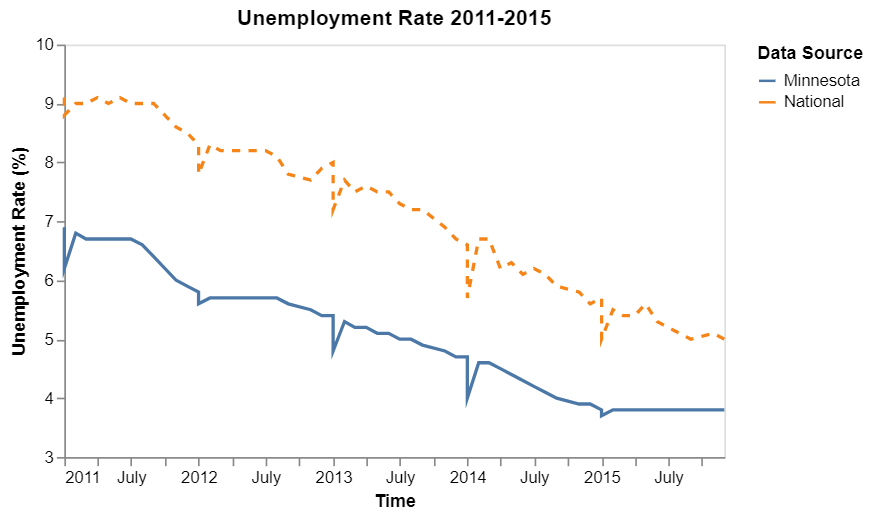
\includegraphics[scale=0.4]{ER.png}
    \caption{Line plot of unemployment rate from 2011 to 2015}
\end{figure} \\
\noindent
For the scatter plot, I try different encodings of three features on both axises and size/color, to minimize influence on the size of graph by outliers. Finally I came up with the parallel plots in Figure 5. \\
\noindent
The position of Minnesota is marked with blue color on the left plot. The dash lines indicate average value of each dimension on the left plot and the value of Red Lake County on the right plot. Both plots share the same y-axis. \\
\begin{figure}[htbp]
    \centering
    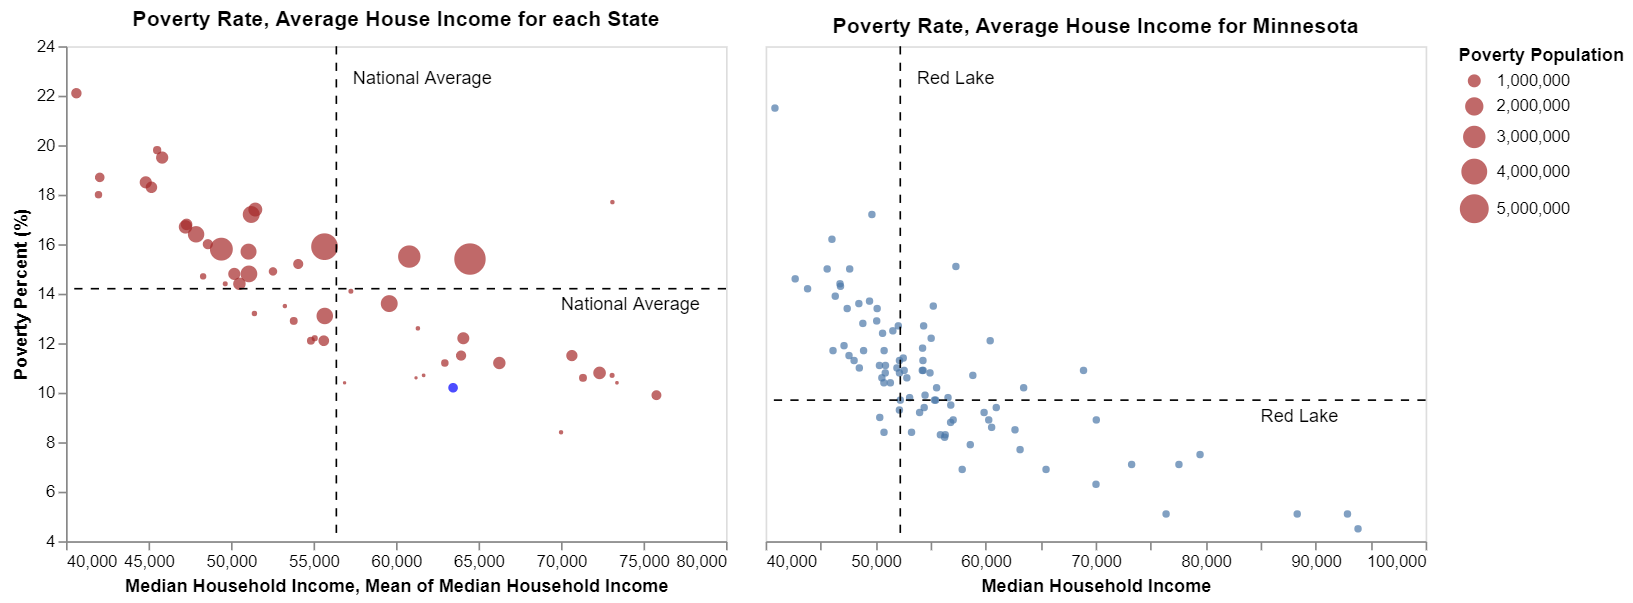
\includegraphics[scale=0.3]{EM.png}
    \caption{Poverty rate, poverty population and household income}
\end{figure}
\newpage
\noindent
As shown in Figure 6, I tried log scale on the x-axis but I think it prevents readers from knowing the real numbers and it makes deviation from average value look smaller for large data. Also, The distance between dots are narrower. \\
\begin{figure}[htbp]
    \centering
    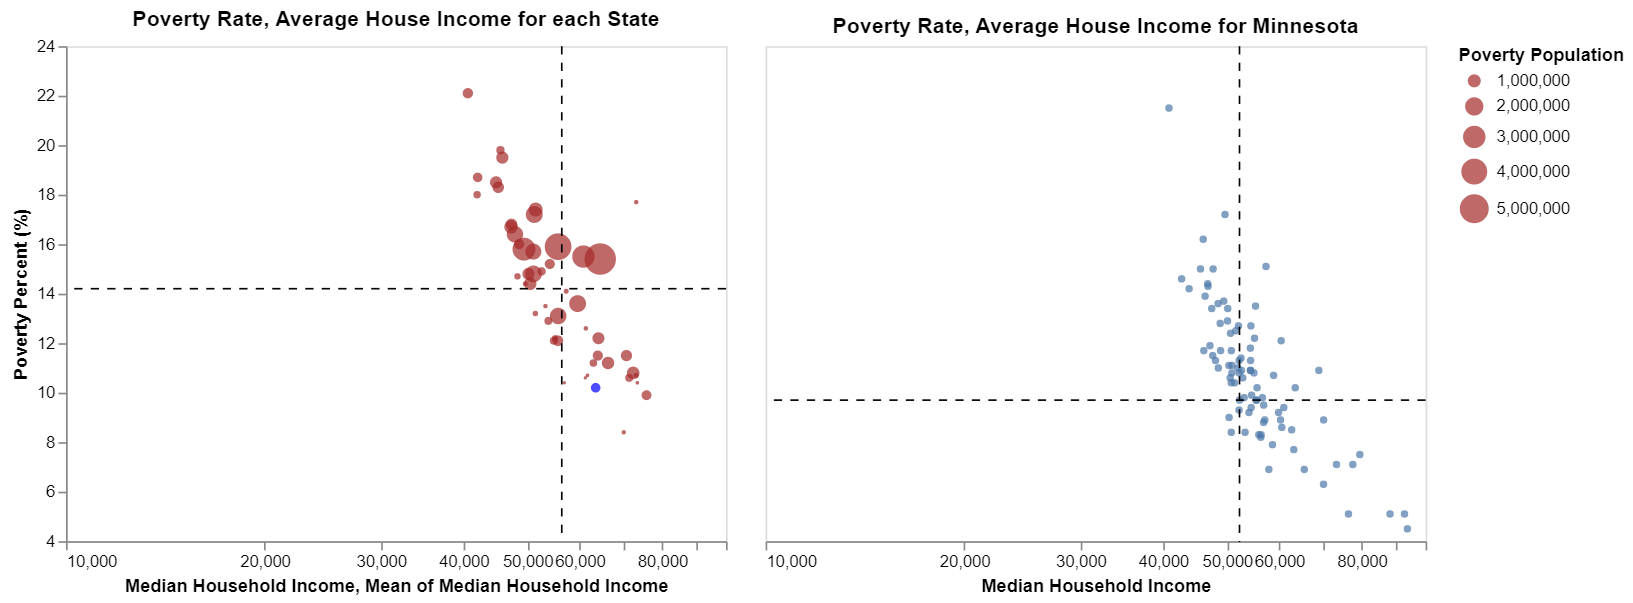
\includegraphics[scale=0.3]{EM_att.png}
    \caption{Poverty rate, poverty population and household income, log scale x-axis}
\end{figure}

\subsubsection*{Bar chart of public school statistics}

As the author mentions education as an important thing in Red Lake County, I decide to contrast the level of educational resources of the county with other counties in Minnesota and the average domestic statistics. I only include data of public schools because there is no private ones in Red Lake. \\
\noindent
I created two calculation fields, one is student per teacher and the other is enrollment rate. A small number of students assigned to each teacher means the educational resources is more abundant. The enrollment rate, which equals to enrollment number divided by the right-age population, is a good indicator of the willingness of pursuing education. The dash lines in Figure 7 stand for national average values. \\
\begin{figure}[htbp]
    \centering
    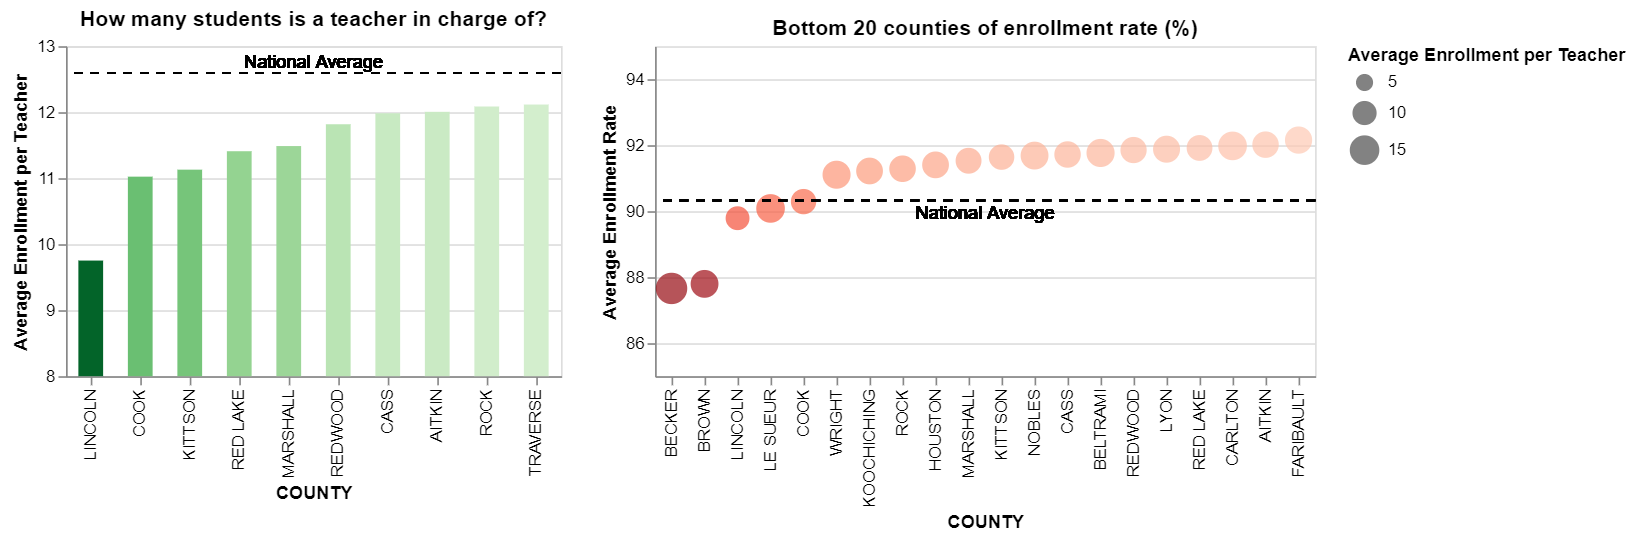
\includegraphics[scale=0.3]{EDU.png}
    \caption{Least enrollment per teacher counties and bottom counties of enrollment rate}
\end{figure}
\newpage
\noindent
What I dislike about the graph is that the size encoding on the right graph is not distinct enough, since the range of average enrollment per teacher is narrow. \\
\noindent
Previously I tried to include the top/bottom 5 values for the left plot in Tableau as Figure 8, but I found there is no necessity and does not add to expressiveness. \\
\begin{figure}[htbp]
    \centering
    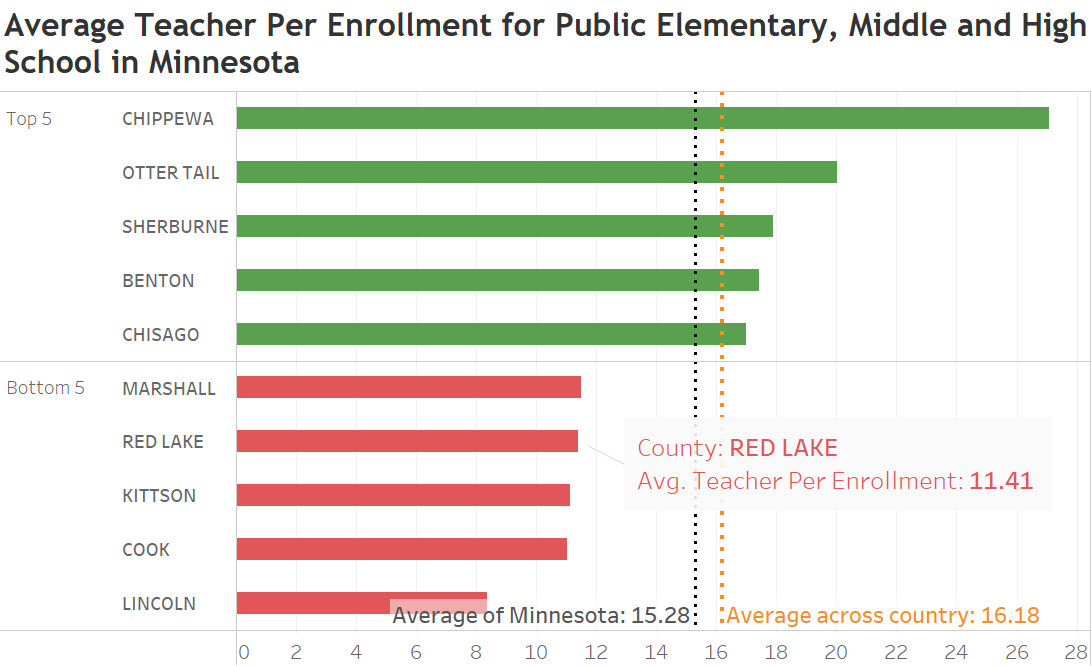
\includegraphics[scale=0.5]{EDU_att.png}
    \caption{Top/bottom 5 counties for enrollment per teacher }
\end{figure}

\subsubsection*{Line \& heatmap plot of mortality}

In this graph, I go a little beyond the content of the article, but I think health is also an important evaluation of whether a place is suitable to live in. I want to see the major diseases causing death and if the health condition improves with time in such a "worst place to live". \\
\noindent
I use a line chart, a scatter plot and a heatmap to display the top 5 mortal diseases in Red Lake and the change of mortality with time. I also make a comparison with national value on the top 5 diseases in Red Lake in terms of the percentage of change in mortality from 1980 to 2014. I like the composed plot as it shows rich information in trend, number, and comparison, together with a good visual effect. \\
\begin{figure}[htbp]
    \centering
    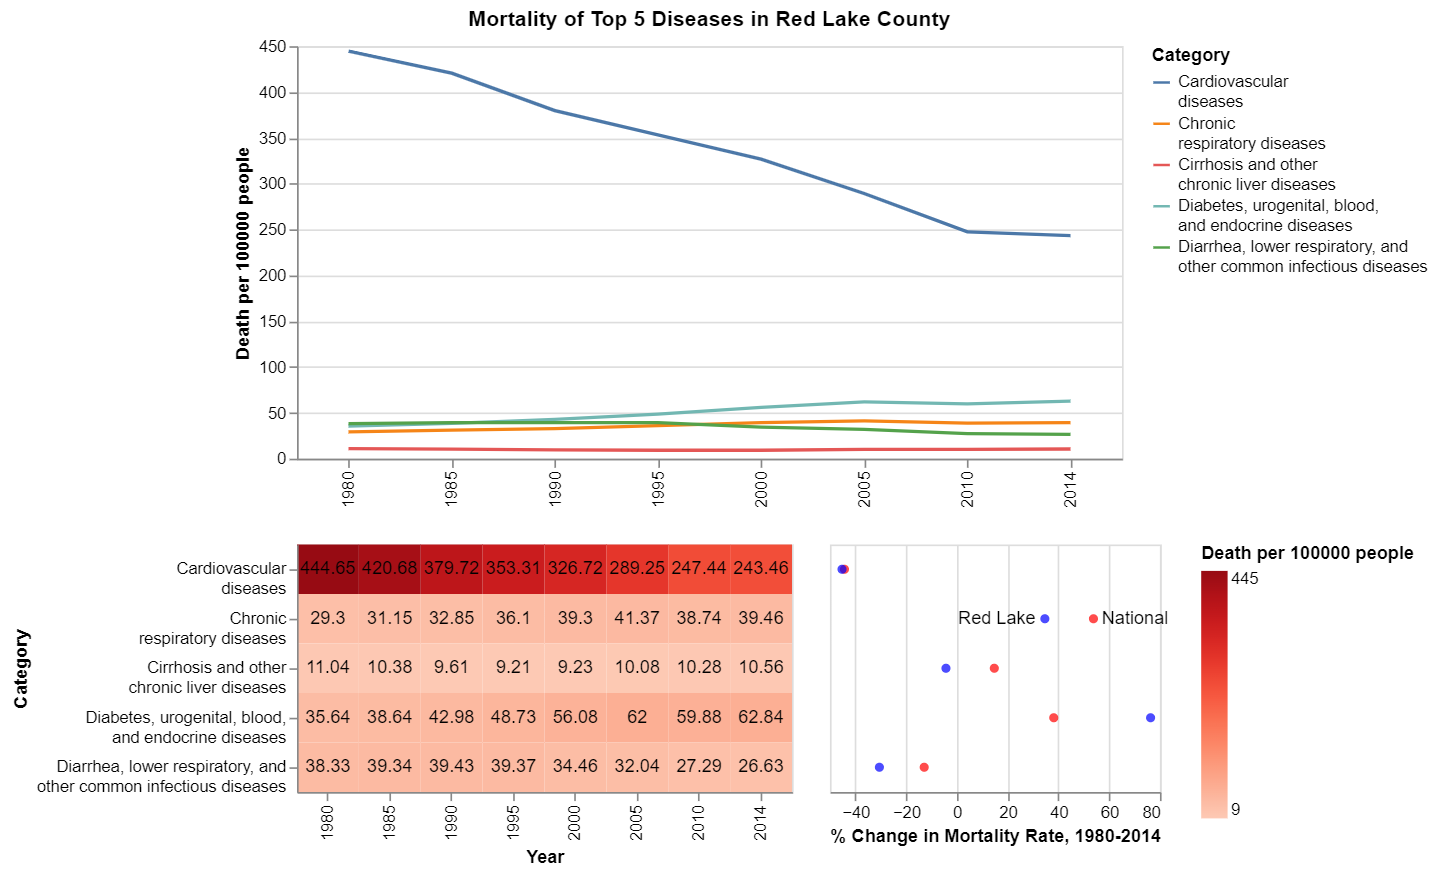
\includegraphics[scale=0.3]{MT.png}
    \caption{Composed plot for top 5 mortal diseases in Red Lake}
\end{figure}
\newpage
\noindent
As the dataset provides min/max values for each year's data, I planned to embed those boundaries into the line chart and the scatter plot, however it appeared too crowdy on the graphs and it is enough for readers to figure out the trends and features of data without knowing the specific ranges.

\section{Final Design}

\begin{itemize}
    \item \textbf{Perception} \\
    Color: I use different color encodings in my visualizations that conform to reader's perception habits. I use green color to encode data containing positive aspects like natural amenity rating and high educational resources. In contrast, red color represents negative data like mortality and bad enrollment rate. For example, higher natural amenity rating leads to darker green (Figure 2), lighter red represents less fatality for a disease (Figure 9). In the scatter plot, there is a color consistency between the highlighted data point on the left graph and dots in the right graph (Figure 5). \\ 
    \noindent
    Cognition: In the scatter plot, I create a pop-out effect using a contrast color to identify the point we want to observe (Figure 5). For multiple lines crossing each other in one chart (Figure 9), color encoding is a good way to reinforce Gestalt Principle of continuity for readers.
    \item \textbf{Design} \\
    Data Ink: I pay careful attention to maximize the data ink ratio in my visualizations. For time-oriented axis (Figure 4, 9.1) and categorical variable axis (Figure 7, 9.3), I erase the grid lines in those dimensions and only leave the grid lines for numerical variables in the purpose of precise reference. Also for the scatter plot (Figure 5), I change the range of both axis to the data range to avoid leaving much blank and make data points sparse on the plot. \\
    \noindent
    Graphic Integrity: All the data in my visualizations are compared and drawn in the same scale, so the lie factors of all graphs are one. I avoid using a logarithm scale on population data to make deviations from mean value different for small and great values, as log scale makes distance between great values narrower. I make necessary annotations for average values (Figure 5, 7), heatmap cells (Figure 9.2), and customized color encodings (Figure 9.3), through bold black font and dash grey lines. All my plots are in 2D, carrying at most three dimensions of data in total, with the extra dimension encoded with color or size. 
    \item \textbf{Interaction}
    (Not decided yet in static version) \\
    \noindent
    The Altair-based graphs are easy to implement interactions on, so I will continue adding features to my graphs to provide efficient and meaningful interactions.
\end{itemize}

\section{Evaluation Method}

To ensure the readers can fulfill my learning object described in the first section, a simple way is to ask a few domain questions about the information we want them to take away, for example:
\begin{itemize}
    \item Which general regions of US have the highest/lowest natural amenity rating?
    \item What diseases have a high death rate for Red Lake County and are there any trends of decrease/increase in mortality with the time? Which diseases did Red Lake County effectively protect against compared to national average after 35 years?
    \item Where is the position of Red Lake County's poverty situation and household income if we put it in a national scale?
    \item What is good about Red Lake County and what is the problem we still need to solve in terms of public education?
\end{itemize}

\noindent
Also a usability test should be done to collect feedback from different users, depending on their social roles, ages, and degree of mastery on reading electronic visualizations. The usability test should be conducted using the control variate method, which means we may only change one factor each time, for example, color encoding, sequence of graph, or annotation font size, to figure out their actual influence on completing the learning objectives.

\end{document}
